\chapter{Memory Management and Pebble Games}

Memory management is important when compiling a program to be run in a resource
constrained environment. It is a topic of great interest in program compilation
in general. The problem is however simpler in the case of irreversible
languages. Once it is determined that some data is no longer needed it can
simply be deleted and reallocated as needed.

In a reversible computation memory management is somewhat complicated by the
reversibility constraint since a bit cannot be simply set to zero and reused
when it is no longer needed. The exact nature of the difference between the
reversible and irreversible memory models is perhaps made most clear by the
rules of the black and reversible pebble games discussed below.

In this section a representation for reversible computation (MDD) is presented.
This representation contains all necessary information about the structure of
the computation that is required for the compiler to perform automated
space-time optimizations using pebble games. It is proposed as an
intermediate representation to be used when compiling high level programming
languages to reversible circuits. 
Such a representation is useful not only in the context of compilation but also in the analysis of circuits.

\section{Overview of Existing Approaches}

\subsection{Janus\label{sec:janus}} 

Janus\cite{YG:2007,LD:1982} is a reversible programming language.  It's main
focus is not to be a circuit description language, but to be logically
reversible. As a result of logical reversibility it does however have some
useful properties which help when compiling to circuits.

Janus guarantees that all programs implemented in it are reversible.
This reversibility is implemented at the statement level, that is to say that
all statements are reversible but the internals of a statement may not be.
This means that temporary ancilla may be allocated to compute a statement but
this ancilla can be cleaned up between statements.

\paragraph{Modification operators} are used for operations that can be done
in-place. For example the addition modification operator, \verb|+=|. Operations
that cannot be done in place can only occur to the right of a modification
operator. These operations can then be implemented, the result can be applied in
place to the left hand side value, and then cleaned up using the Bennett method if
necessary. This means that memory need only be allocated temporarily for each
modification statement.

For example say we wish to evaluate the statement \verb|b+=a*c|\footnote{i.e.
replace the bit-string $b$ with the value $b+ac\mod 2^n$ where $n$ is the
length of $b$.}. First \verb|a*c| is computed by using additional ancilla as
needed. The result is then reversibly added to \verb|b| (using the function
$(a,b)\mapsto(a,a+b)$ discussed previously). Finally the circuit for \verb|a*c|
can be reversed in order to clean up any allocated ancilla.

\paragraph{If conditions} require a pre-condition which is used to choose which
branch to take, and a post-condition which is true if and only if the top
branch is taken). These are very useful\todo{explain with example} in the
context of memory management. The pre-condition can be used to set a bit which
controls which operations are performed. The post-condition can be used to
clear this bit as the pre-condition may no longer be true after the loop is
performed.

\todo{add diagram}

\subsection{Pebble Games}

Any computation where execution is independent of input can be modeled as a
Directed Acyclic Graph (DAG). This graph is sometimes called a
\emph{Functional-dependence} network.  The nodes on the graph are associated
with functions and the arrows represent data dependencies required for the
computation of those functions. These graphs are loop free by construction
assuming \todo{Clarify} no circular dependencies.

The \emph{Black Pebble Game} is a game played on a DAG which is used to model
irreversible computation. The rules are as follows:\todo{Example!}

\begin{enumerate}
  \item A pebble can be added to a node if and only if all predecessors of the
    node have pebbles.
  \item A pebble can be removed at any time.
\end{enumerate}

Pebble games are often used to study space-time trade-offs in computing. For
example if we take some computation and model it as a DAG we can try and find
the minimum number of pebbles needed to compute some value in the graph. This
minimum corresponds to the minimal space cost of that computation.

To model a computation as a DAG draw nodes representing a single register state
in the computation.  These nodes are then connected based on data dependencies.
Any computation which is valid (does note contain circular dependencies) will
form a DAG using this procedure.

\subsubsection{Reversible Pebble Game}

Bennett\cite{Bennett:89} describes an alternative pebble game for reversible
computation. The rules are similar to those used in the \emph{black pebble
game} except that the reversibility constraint prevents us from simply removing
pebbles. Each computation has a corresponding reverse computation, and the
dependencies of the reverse computation are the same as the corresponding
forward computation. This means that pebbles may still be removed, but removal
is subject to the same conditions as placement. In other words we make
placement and removal of pebbles symmetric similarly to the way forward and
reverse computation are made symmetric in reversible computing.  The rules for
this version of the game are given below:\todo{Example!}

\begin{enumerate}

  \item A pebble can be added to a node if and only if all predecessors of the
    node have pebbles

  \item A pebble can be removed from a node if and only if all predecessors of
    the node have pebbles

\end{enumerate}

The space complexity of a game is given by the maximum number of pebbles which
are in play at any given time. It has been shown that in general computing the
\emph{pebble number} (the minimum number of pebbles, over all possible games,
required to the final target pebble) for an arbitrary DAG is
PSPACE-complete\cite{chan13} \todo{for a physics thesis, you at least need a
footnote explaining what this is, and relate to NP-complete, since this is more
familiar in physics. and mention that it also contains BQA, QMA, and it's
generalization QIP, which in fact equals PSPACE.}.

Strategies for playing these games have been analyzed in the case of, one
dimensional directed graphs, as well as for trees\cite{peb16}.  There are three
particular strategies of interest in the simple 1D case where all nodes have
equal cost (\cref{fig:pebble} represents these strategies visually):

The first is the naive strategy (sometimes called \emph{Bennett Method}). In
this strategy pebbles are added one after another until the desired pebble is
reached.  All of the extra pebbles used in the computation are then removed in
reverse order. This strategy has time complexity $2n-1$ and space complexity
$n$. This is the minimal time strategy in the 1D graph. The equivalent strategy
on a general DAG might be to fill in all pebbles in topological order then
remove all non-output pebbles in reverse order.

The second is a slightly more advanced strategy which will be referred to as
the \emph{incremental strategy}. Here we start with some limited number of
pebbles and place pebbles until we run out. After running out we uncompute all
but the last pebble following the Bennett strategy. This is then repeated using
the next pebble as the new starting point until the desired pebble is reached.
This strategy has a time complexity of $O(n)$ and a space complexity of
$O(\sqrt n)$. This means that we can can get a square root reduction in space
in exchange for a constant multiplier on time, therefore the asymptotic
space-time product of the circuit can be improved over the naive strategy.
Although this strategy is not optimal in all cases it is easy to implement due
to not requiring that the cleanup algorithm have prior knowledge about the size
of the circuit. A similar strategy applied to trees is used in \cref{sec:kara}
in the analysis of reversible Karatsuba.

Finally the third is the optimal strategy (for a given space bound) from Knill
\cite{knill:95}. Finding such a strategy in the general case is
PSPACE-complete.  

\todo{Briefly explain Knill}

\todo{Add a section about pebble games on trees and their relationship with reversible functions.}

\begin{figure}
  \centering
  \begin{subfigure}{0.3\textwidth}
    \centering
    
\includegraphics{images/Pebble1.png}
    \caption{Bennett Method}
  \end{subfigure}
  \begin{subfigure}{0.3\textwidth}
    \centering
    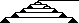
\includegraphics{images/Pebble2.png}
    \caption{Incremental}
  \end{subfigure}\begin{subfigure}{0.3\textwidth}
    \centering
    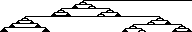
\includegraphics{images/Pebble3.png}
    \caption{Knill}
  \end{subfigure}
  \label{fig:pebble}
  \caption{Comparison of 1D pebble strategies. The horizontal axis represents
  time and the vertical axis is the state of the game at a given time slice.}
\end{figure}

\section{Mutable Dependency Diagram(MDD)}
\todo{This name should probably be changed to imply that this is a game.}

In this section a new game for the optimization of reversible computation is
presented. It is a generalization of the reversible pebble game in that any
reversible pebble game can be represented on an MDD. 

Lacking in the original pebble game is an effective way to represent
mutation\footnote{Mutation in this context means variables that change in
value. For example the modification operators operators discussed above in
\cref{sec:janus}}. This is of not much consequence in the irreversible pebble
game since mutation can be modeled as a placement followed by the removal of a
dependency. In the reversible pebble game it is significantly more important
since pebbles can normally only be removed if predecessors are pebbled. For
example addition via the mapping $(a,b) \mapsto (a,a+b)$ (implemented by an
in-place addition circuit) is a reversible operation which does not require new
space to be allocated for the result $a+b$.  In order for strategies from the
reversible pebble game to be applied to a circuit using this operation
generically it would have to be made out of place by copying the $b$ input and
thus losing the advantages that may have been gained by using an in-place
operation.

In order to better represent in-place operations a new pebble game is proposed.
Rules one and two are similar to the reversible pebble game. The third rule
(as well as two types of labeled edges) has been added:\todo{Example!}

\begin{enumerate}

   \item A new pebble can be added to a node if and only if all predecessors of
     the node have pebbles.

   \item A pebble can be removed from a node if and only if all predecessors of
     the node have pebbles.

   \item A pebble may be moved forward or backward along a mutation edge if all
     predecessors of the node to which the edge points have pebbles.

\end{enumerate}

Note that since using the move described in the third rule is optional this is
a generalization of the reversible pebble game and any strategy that can be
used in the reversible pebble game is a valid strategy here. We also inherit
the PSPACE-completeness (\cite{chan13}) of solving the reversible pebble game
since any graph which does not include mutation edges is played by the rules of
the reversible pebble game. This means that in general solving an MDD must be
at least as hard.

As a simple example of the usefulness of such a game consider the computation
of $a+b+c$. In \cref{fig:mddExample} the reversible pebble graph as well as the
MDD are given. If the inputs ($a$,$b$,$c$) are considered to be pebbled then
two additional stones to pebble $a+b+c$ in the reversible pebble game. The
first pebble is placed on $a+b$ and the second can then be placed on $a+b+c$.
The MDD game on the other hand does not need any additional stone. In the MDD
the $b$ stone can be slid along the modification path to $a+b$ then further
slid along to $a+b+c$. So it is possible to use two fewer stones (no additional
stones beyond the inputs) in the MDD game. Note that since this game is a
generalization of the reversible pebble game the best strategy for an MDD will
always be equivalent to or better then the best strategy in the corresponding
reversible pebble game.

\begin{figure}
  \centering
  \begin{subfigure}{0.3\textwidth}
    \includegraphics{images/revPeb.tikz}
    \caption{Reversible}
  \end{subfigure}
  \qquad\qquad
  \begin{subfigure}{0.3\textwidth}
    \includegraphics{images/mddPeb.tikz}
    \caption{MDD}
  \end{subfigure}
  \label{fig:mddExample}
  \caption{The reversible pebble game and MDD for $a+b+c$. Mutation edges are
  represented with sold lines while normal dependency edges used a dashed line.}
\end{figure}


\subsection{Converting a Computation to an MDD}

First I will define the elements of the graph in terms of what they represent
with respect to computation:

\paragraph{Nodes} represent a register in some state.

\paragraph{Mutation Edges} represent operations which transform the value
of a register. The parent and child node of an edge represent the state of the
register before and after (respectively) the computation. Each node may have
only a single input and output mutation edge. A chain of nodes connected by
mutation edges represents all computations which change the contents of a
register.

\paragraph{Dependency Edges} point from values upon which a computation
depends. In order for a computation defined by a mutation edge to be implemented
all parent nodes along dependency edges pointing to the child node of the
mutation edge must be available.

For example the computation $(a,b)\mapsto(a,a+b)$ might be represented as a
solid arrow from the node $b$ to the node $a+b$ with a dependency arrow coming
from $a$.


\begin{theorem} For all MDDs a strategy to pebble all nodes exists and is
efficiently computable. \end{theorem}

\begin{proof} Consider the following simple strategy. First perform a
topological sort\footnote{A topological ordering is an ordering of nodes in
a graph such that for all edges $ab$; $a$ comes before $b$. A DAG
always has at least one topological ordering. The complexity of finding
a topological (i.e. performing a topological sort) ordering is $O(E+V)$
where $E$ is the number of edges and $V$ is the number of vertices in the
graph.} on the nodes of the graph. Now place a pebble on each node in the
sorted order. It is guaranteed that the dependencies of each node will be
pebbled since they are placed in sorted order. The entire graph may be covered
by pebbles in this fashion.\end{proof}

\todo{Other things that may be nice to prove, the construction of an MDD from a
      simple language show that the MDD computes the same function as the language.}

\todo{Show how conversion from Janus allows for temporary variables while
maintaining all implicit cleanup from the original language}


\subsection{Computing the Cost of a Strategy}

In order to compute the cost of a given strategy a few additional rules are
needed:

\begin{enumerate}
    \setcounter{enumi}{3}
  \item Each node has a computation cost which is payed when placing a new pebble on
    it or sliding an existing pebble to it.
  \item Each node has a space cost which gives the contribution of that node to
    the overall space complexity when it is pebbled.
  \item If a node has no parent it computes a constant so a pebble may be placed
    at any time.
\end{enumerate}

A implementation of a computation can be represented by an MDD and a list of
moves $\{m_i:i \in 1 \dotsc n\}$ (where $n$ is the total number of moves making up the
computation) where each move consists of a graph location and a move type. Given
a function $C$ which returns the gate cost of a move the total gate cost of a
computation is then:
\[ \sum_{i\in 1 \dotsc n} C(m_i) \]

Another way to represent the computation is as a set of states representing the
graph after each move $\{g_i:i \in 1 \dotsc n\}$. Given a function $S$ which
returns the total space in use for a state (by summing over the cost of all
currently placed pebbles) we can compute the space complexly as:

\[ \max_{i\in 1 \dotsc n} S(g_i) \]

The goal of this game is to come up with a set of moves the minimizes the total
movement cost as well as the space complexity.

When implementing the graph as a circuit we may perform the computations in any
valid topological ordering. Further if there are multiple computations which
could be next in a given ordering they can be performed in parallel.

Some heuristic strategies are discussed below.

\subsection{Eager Cleanup}

If a value is no longer needed in a computation it can then be checked that the
information needed to clean it up is \emph{available}. Available is defined to
mean that all dependencies needed to move the pebble to the beginning of its
modification path currently have pebbles or have pebbles that can be moved into
place (by sliding along mutation edges) without causing additional space to be
used. If this is the case it can immediately be cleaned and the ancilla can be
freed for future use in the computation.

Eager cleanup is possible when all dependencies are \emph{one-way}.
This means that once there is no path from it to any of the modification paths
of its dependencies (as shown in \cref{fig:one-way}).

\begin{figure}
  \centering
  \begin{subfigure}[b]{0.3\textwidth}
    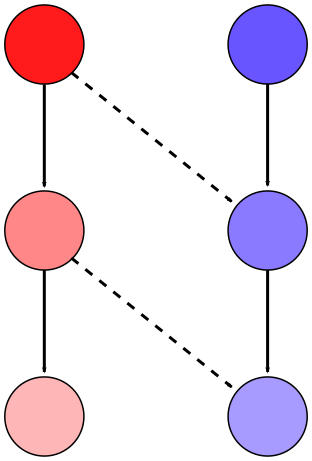
\includegraphics[width=0.8\textwidth]{images/oneway.pdf}
    \caption{One Way}
    \label{fig:one-way}
  \end{subfigure}
  \qquad
  \begin{subfigure}[b]{0.3\textwidth}
    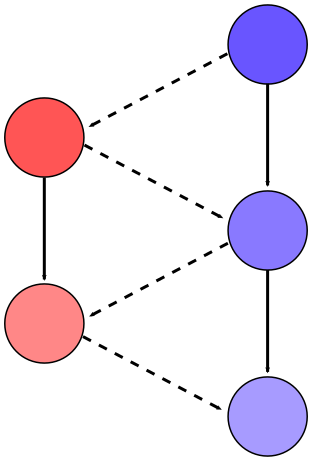
\includegraphics[width=0.8\textwidth]{images/interdependent.pdf}
    \caption{Interdependent}
    \label{fig:interdep}
  \end{subfigure}
  \caption{Dependency patterns which effect eager cleanup}
\end{figure}

\todo{Write algorithm out formally and adapt the below proof sketch to the neewversion}

\begin{theorem}

Eager cleanup is possible on any graph with only one-way dependencies.  Let
$G=(V,E)$ be an MDD.  Assume that all mutation paths in $G$ are one-way
dependent\todo{define this}.\textsc{Eager} cleanup method in Algorithm
\ref{alg:eager}\todo{Add this algorithm} is correct in the sense that it all
ancillas that may be used by ${\mathcal C}$ are returned in their initial state
at the end of the computation.

\end{theorem}

\begin{proof}
  \todo{This proof might be better with a diagram}

Consider a graph which consists of one-way dependent paths $P_1,\dotsc,P_n$
arranged in topological order. Assume that for a $P_k$ we can move the pebble
in each path to an arbitrary position on the path.

For the base $k=1$ there is only one mutation path, this path either leads to
an output, in which case no cleanup is necessary, or leads to a node that has
to be cleaned up. However, since all inputs to the path are still available by
assumption, the pebble on this path may be moved up and down and may therefore
be moved to an arbitrary position. 

Now, we make the inductive step to $k+1$ paths. Recall that a pebble can be
moved backward along a path if all their dependency edges pointing to the node
that it occupies point from nodes which contain pebbles. We therefore make the
inductive step as follows: by assumption on the one-wayness of the graph, all
edges point into $P_{k+1}$ and none points backward. Now, consider all nodes in
$P_1, \ldots, P_k$ that would have to be pebbled in order to move the pebble on
path $P_{k+1}$ one step backward or forward. By induction, starting with $P_k$,
we can slide the pebbles on each path into the location that is needed to move
the pebble on $P_k$. By repeating this we may move the pebble on $P_{k+1}$ to
any location on the graph.

\end{proof}

\subsection{Triangles and Incremental Cleanup}

\Cref{fig:interdep} shows a graph where eager cleanup fails. The red mutation
path depends on previous values of the blue path in order to be cleaned.

It is still possible to clean up the blue node. A method for doing this is
somewhat related to the \emph{incremental strategy} discussed above generalized
to a DAG.

In this strategy we start adding filling in pebbles working toward the final
pebble. After we have placed a certain number of pebbles (up to some space
limit we are trying to achieve), we stop and find the set of the currently
pebbled nodes that are dependencies of future nodes. We then create a
'checkpoint' removing all nodes except the ones in this set by reversing the
computation.  Using the newly freed up pebbles the computation can be
continued.  If we run out of pebbles again we can create a new checkpoint and
remove all pebbles up to the previous one and so on. Note that it is helpful to
choose checkpoint locations where the set of nodes with future dependencies is
small.

This strategy introduces a constant multiplier on time in exchange for a
quadratic reduction in space in some cases. This is not necessarily the case
for all all graphs. Later discussion in \cref{sec:kara} shows a smaller then
quadratic space reduction in the case of a specific graph. See \cref{sec:kara}
for an application of this strategy to the Karatsuba circuit.

\subsection{Circuit Generation}

Circuit generation is defined by creating a generation function for each type
of move allowed in the game then using that set of functions to convert a graph
and move set into a circuit. When using an MDD to construct a circuit additional
information must be added to each node specifying which circuit input
corresponds to each incoming arrow.

We start with a circuit consisting of registers corresponding to the input
nodes of the graph, these are the inputs to the circuit. A heap\todo{Explain}
of currently available ancilla is kept. This ensures that the lowest available
numbered ancilla is always the one allocated so ancilla use is minimized.

Starting with a set of built in functions, new functions can be constructed as MDDs.
After a function is constructed it can be used a graph node in an MDD.

\begin{itemize}

    \item Place Pebble: Place circuit which computes the function at the node
	    using the nodes dependencies as input. Assign ancilla for the
	    output of the circuit from the heap.

    \item Remove Pebble: Place the reverse circuit for the function at the node
	    using dependencies as input, uncomputing the previously computed
	    value.  Return previously assigned ancilla to the heap (ancilla
	    assigned when the pebble was placed).

    \item Slide Pebble: Place circuit which computes the function at the node
	    using the nodes dependencies as immutable input and the bits representing the
	    current value of the node as the modified input.

\end{itemize}

\todo{Example: Extracting an MDD and generating a circuit for a simple Janus program.}

\todo{prove, under some assumptions, that this procedure constructs a circuit
        computing the same function as the MDD }

\subsection{Example: SHA-256 Round}

A simple statement of the computation done in one round of SHA-256 is given in
\cref{alg:sha2}. A direct translation of this algorithm into an MDD is given in
\cref{fig:sha-MDD}.  One immediate advantage of the representation is that
computation on the $h$ and $d$ registers may be modified rather then reassigned
at each step. It can also be seen from the MDD that the computed temporary values
(Maj, Ch, $\Sigma_0$,$\Sigma_1$) all have one way dependencies and depend only
on unmodified input values. The can therefore be cleaned up directly after they
are used using the eager cleanup scheme. The resulting circuit is shown in
\cref{fig:sha}.

\begin{algorithm}
\caption{SHA-256}
\label{alg:sha2}
\begin{algorithmic}
  \For{$i \gets 0, 63$}
    \State \hspace*{1em} $\Sigma_1 = (\mathbf{E} \ggg 6) \oplus (\mathbf{E} \ggg 11) \oplus  (\mathbf{E} \ggg 25)$
    \State \hspace*{1em} $\mathbf{Ch} = (\mathbf{E} \land \mathbf{F}) \oplus ( \neg\mathbf{E}\land \mathbf{G})$
    \State \hspace*{1em} $\Sigma_0 = (\mathbf{A} \ggg 2) \oplus (\mathbf{A} \ggg 13) \oplus (\mathbf{A} \ggg 22)$
    \State \hspace*{1em} $\text{Maj} = (\mathbf{A} \land \mathbf{B}) \oplus (\mathbf{A} \land \mathbf{C}) \oplus (\mathbf{B}\land\mathbf{C})$
    \State \hspace*{1em} $\mathbf{H} \pluseq \Sigma_1 + \mathbf{Ch} + \mathbf{K}[i] + \mathbf{W}[i]$
    \State \hspace*{1em} $\mathbf{D} \pluseq \mathbf{H}$
    \State \hspace*{1em} $\mathbf{H} \pluseq \Sigma_0 + \text{Maj}$
  \EndFor
\end{algorithmic}
\end{algorithm}

\begin{figure}
      \capstart
      \centering
      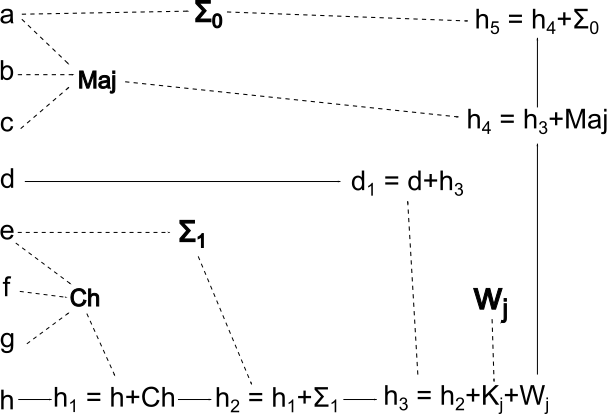
\includegraphics[width=0.7\hsize]{images/sha_MDD}

      \caption{MDD for one round of SHA-256 generated using the eager cleanup
      method. Note for example that a pebble can be placed on $\mathbf{Ch}$ and
      then removed after $\mathbf{h}_1 = \mathbf{h}+\mathbf{ch}$ is computed}

      \label{fig:sha-MDD}
\end{figure}

Note that the order of operations chosen for the circuit could have different
based on the MDD. The compiler is allowed to exploit any ambiguity allowed by
the representation to implement more optimized circuits.

\begin{figure}
      \capstart
      \centering
      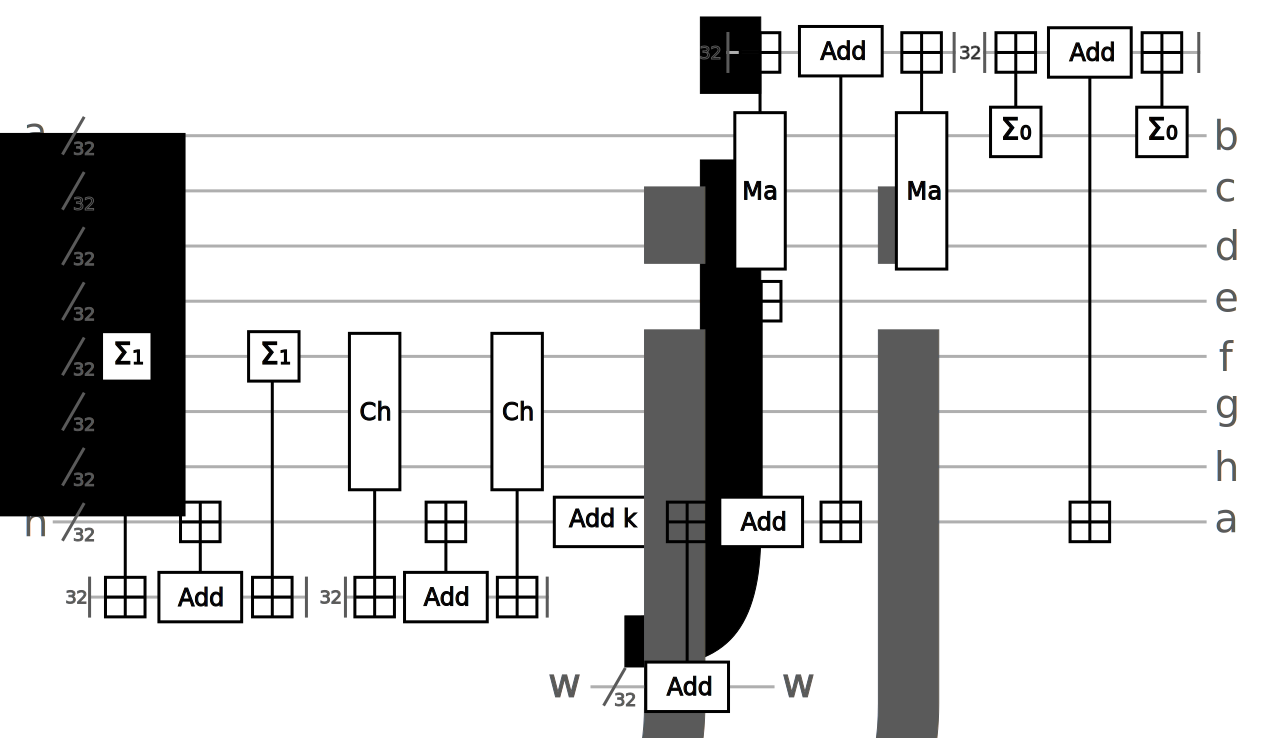
\includegraphics[width=0.9\hsize]{images/sha_round}
      \caption{One Round of SHA-256}
      \label{fig:sha}
\end{figure}

\section{Discussion and Open Problems} 

Heuristic methods for playing the pebble game on a general DAG were presented.
It is likely that there exist efficiently computable methods with better time
and/or space performance.  

Additionally methods for the conversion of other reversible languages to an MDD
intermediate might give further insight into the types of useful heuristic
strategies that might be implemented. It would also be interesting to explore
MDD games on some special graphs which correspond to common computations.
